\documentclass[12pt, a4paper]{article}
\usepackage[utf8]{inputenc}
\usepackage{array}
\usepackage[spanish]{babel} 
\usepackage[margin=1.8cm]{geometry}
\usepackage{graphicx}

\newcolumntype{C}[1]{>{\centering\arraybackslash}m{#1}}
\newcolumntype{L}[1]{>{\raggedright\arraybackslash}m{#1}}

\begin{document}

 %==================== CU-001 ====================
\begin{center}
\begin{tabular}{
  |>{\centering\arraybackslash}m{4cm}|
   >{\centering\arraybackslash}m{5cm}|
   >{\centering\arraybackslash}m{4cm}|
   >{\centering\arraybackslash}m{3cm}|
}
\hline
\textbf{Código de caso de uso} & CU-001 & \textbf{Nombre del Caso de Uso} & Iniciar sesión \\
\hline
\textbf{Actor principal} & Administrador / Vendedor & & \\
\hline
\textbf{Actor Secundario} & Ninguno & & \\
\hline
\textbf{Descripción} & \multicolumn{3}{>{\centering\arraybackslash}m{12cm}|}{Permite a un usuario registrado autenticarse en el sistema para acceder a las funcionalidades según su rol.} \\
\hline
\textbf{Precondiciones} & \multicolumn{3}{>{\centering\arraybackslash}m{12cm}|}{El usuario debe estar registrado y activo en el sistema.} \\
\hline
\textbf{Postcondiciones} & \multicolumn{3}{>{\centering\arraybackslash}m{12cm}|}{El sistema crea una sesión activa para el usuario. \newline El sistema registra la fecha y hora de inicio de sesión. \newline Se cargan los permisos correspondientes al rol del usuario.} \\
\hline
\multicolumn{4}{|>{\centering\arraybackslash}m{15.7cm}|}{\textbf{Flujo Principal}} \\
\hline
\multicolumn{2}{|C{8cm}|}{\textbf{Acción del actor}}
& \multicolumn{2}{C{8cm}|}{\textbf{Respuesta del Sistema}} \\
\hline
\multicolumn{2}{|C{8cm}|}{1. Ingresa usuario y contraseña.}
& \multicolumn{2}{C{8cm}|}{Valida credenciales contra la base de datos.} \\
\hline
\multicolumn{2}{|C{8cm}|}{2. Confirma el inicio de sesión.}
& \multicolumn{2}{C{8cm}|}{Crea la sesión, carga permisos y redirige al panel principal.} \\
\hline
\multicolumn{4}{|C{15.7cm}|}{\textbf{Flujos Alternativos}} \\
\hline
\multicolumn{2}{|C{8cm}|}{A1}
& \multicolumn{2}{C{8cm}|}{Credenciales incorrectas. Muestra mensaje ``Usuario o contraseña incorrectos'' y permite reintentar.} \\
\hline
\multicolumn{2}{|C{8cm}|}{A2}
& \multicolumn{2}{C{8cm}|}{Cuenta bloqueada por intentos fallidos. Muestra mensaje ``Cuenta bloqueada. Contacte al administrador.''} \\
\hline
\multicolumn{4}{|C{15.7cm}|}{\textbf{Flujos de Excepciones}} \\
\hline
\multicolumn{2}{|C{8cm}|}{E1}
& \multicolumn{2}{C{8cm}|}{Fallo de conexión con el servicio de autenticación. Muestra mensaje ``Servicio no disponible. Intente más tarde.''} \\
\hline
\textbf{RF asociados} & RF-10, RF-11 & \textbf{RNF asociados} & RNF-02 \\
\hline
\end{tabular}
\end{center}

\newpage

\subsection*{Diagrama de caso de uso ``CU001''}
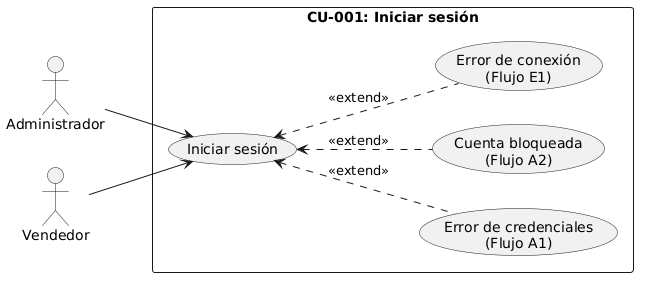
\includegraphics[width=0.9\textwidth]{doc/imagenes/Diagrama_de_Casos_de_Uso_CU001.png}
 
\end{document} 
